\documentclass{beamer}
\beamertemplatenavigationsymbolsempty
\usepackage{mathtools,amsmath,amssymb,amsfonts}
\usepackage{tikz,scalerel,pict2e,tkz-euclide,tikz-3dplot}
\usepackage[dvipsnames]{xcolor}
\usetikzlibrary{calc,patterns,arrows.meta,shadows,external,spath3}
\usetikzlibrary{decorations.pathreplacing,angles,quotes,perspective,intersections}
\usepackage{pgfplots}
\pgfplotsset{compat=1.18}
\usepgfplotslibrary{statistics,fillbetween}

\pgfplotsset{
    standard/.style={
    axis line style = thick,
    trig format=rad,
    enlargelimits,
    axis x line=middle,
    axis y line=middle,
    enlarge x limits=0.15,
    enlarge y limits=0.15,
    every axis x label/.style={at={(current axis.right of origin)},anchor=north west},
    every axis y label/.style={at={(current axis.above origin)},anchor=south east}
    }
}
\newcommand{\Vn}{360}
\begin{document}
\begin{frame}
\centering
\tdplotsetmaincoords{0}{90}
\begin{tikzpicture}[tdplot_main_coords]
\draw[white,tdplot_main_coords] (-4.5,-3.5) rectangle (4.5,5);
\tdplotsetrotatedcoords{0}{0}{0}
\draw[tdplot_rotated_coords,domain=90:\Vn,smooth,very thin,samples=5000,variable=\Vt] plot ({sqrt(1-(\Vt/360)^2)*sin(40*\Vt)/(1-sqrt(1-(\Vt/360)^2)*cos(40*\Vt)))},{(\Vt/360)/(1-sqrt(1-(\Vt/360)^2)*cos(40*\Vt))*cos(3*\Vt)},{(\Vt/360)/(1-sqrt(1-(\Vt/360)^2)*cos(40*\Vt))*sin(3*\Vt)});
\end{tikzpicture}
\end{frame}

\begin{frame}
\tdplotsetmaincoords{0}{0}
\begin{tikzpicture}[tdplot_main_coords, scale=1.5]
\draw[tdplot_screen_coords] (0,0) circle [radius=1];
\foreach \t in {0, 10, ..., 350}{
\begin{scope}
%\clip[] (-2,-2,0) rectangle (2,2,2);
\tdplotsetrotatedcoords{0}{\t}{0}
\draw[tdplot_rotated_coords,very thin] (0,0) circle [radius=1];
\tdplotsetrotatedcoords{90}{90}{0}
\draw[tdplot_rotated_coords,very thin] (0,0,{sin(\t)}) circle [radius={cos(\t)}];
\end{scope}}
\end{tikzpicture}
\end{frame}

\begin{frame}
\tdplotsetmaincoords{55}{60}
\begin{tikzpicture}[tdplot_main_coords, scale=1]
\draw[rotate=30] (-4,-4,0) -- (-4,2.2,0) -- (7,2.2,0) -- (7,-4,0) -- cycle;
\node at (0.8,-5,0) {$\overline{\mathbb{C}}$};
\draw[-latex] (0,0,-3) -- (0,0,2); % z-axis
\draw[tdplot_screen_coords] (0,0) circle [radius=1]; % outer circle
\tdplotsetrotatedcoords{0}{0}{0}
\draw[tdplot_rotated_coords] (0,0) circle [radius=1]; % base intersection
\tdplotsetrotatedcoords{0}{21.8}{0}
\path[tdplot_rotated_coords,spath/save=PcircS] (0,0) circle [radius=0.3714];
\path[tdplot_rotated_coords,spath/save=PcircL] (0,0) circle [radius=0.3714];
\path[fill,opacity=0.5,spath/use={PcircS, transform={shift={(1*0.35582,1*0,1*0.862)}}}]; % NOTE: we swapped x and y for simplicity
\path[draw,spath/use={PcircS, transform={shift={(1*0.35582,1*0,1*0.862)}}}]; % NOTE: we swapped x and y for simplicity
\draw[] (2.5,-3) -- (2.5,2);
\draw[very thin] (0,0,1) -- (2.5,-2.2,0);
\draw[very thin] (0,0,1) -- (2.5,1.5,0);
\draw[very thin] (0,0,1) -- (2.5,0,0);
\node[left] at (0,0,1) {$\scriptscriptstyle N$};

\end{tikzpicture}
\end{frame}

\begin{frame}
\tdplotsetmaincoords{55}{10}
\begin{tikzpicture}[tdplot_main_coords, scale=1]
\draw[] (-2,-4,0) -- (-2,3,0) -- (6,3,0) -- (6,-4,0) -- cycle;
\node at (-1.6,-3.2,0) {$\overline{\mathbb{C}}$};
\draw[-latex] (0,0,-2) -- (0,0,2); % z-axis
%\draw[-latex] (-2,0,0) -- (7,0,0) node[pos=1,above right]{$y,\zeta$}; % y-axis (swapped with the x for simplicity)
\draw[tdplot_screen_coords] (0,0) circle [radius=1]; % outer circle
\tdplotsetrotatedcoords{0}{0}{0}
\draw[tdplot_rotated_coords] (0,0) circle [radius=1]; % base intersection
\tdplotsetrotatedcoords{0}{37.87}{0}
\path[tdplot_rotated_coords,spath/save=PcircS] (0,0) circle [radius=0.26];
\path[tdplot_rotated_coords,spath/save=PcircL] (0,0) circle [radius=0.26];
\path[fill,opacity=0.5,spath/use={PcircS, transform={shift={(1*0.5923,1*0,1*0.7615)}}}]; % NOTE: we swapped x and y for simplicity
\path[draw,spath/use={PcircL, transform={shift={(1*0.5923,1*0,1*0.7615)}}}]; % NOTE: we swapped x and y for simplicity
\draw[fill,opacity=0.5] (3.5,0) circle [radius=1.5];
\draw[] (3.5,0) circle [radius=1.5];
\draw[very thin] (0,0,1) -- (3.5,0,0);
\draw[very thin] (0,0,1) -- (3.5,-1.5,0);
\draw[very thin] (0,0,1) -- (3.5,1.5,0);
\draw[very thin] (0,0,1) -- (2,0,0);
\node[left] at (0,0,1) {$\scriptscriptstyle N$};
\draw[fill,opacity=0.5] (0,0) circle [radius=0.26];
\path[spath/save=PcircS] (0,0) circle [radius=0.4877];\
\path[fill,opacity=0.5,spath/use={PcircS, transform={shift={(1*0,1*0,1*-0.873)}}}]; % NOTE: we swapped x and y for simplicity
% intersection circle\
\draw[very thin,dashed] (0,0,1) -- (0.4877,0,-0.873);
\draw[very thin,dashed] (0,0,1) -- (-0.4877,0,-0.873);
\end{tikzpicture}
\end{frame}


\begin{frame}
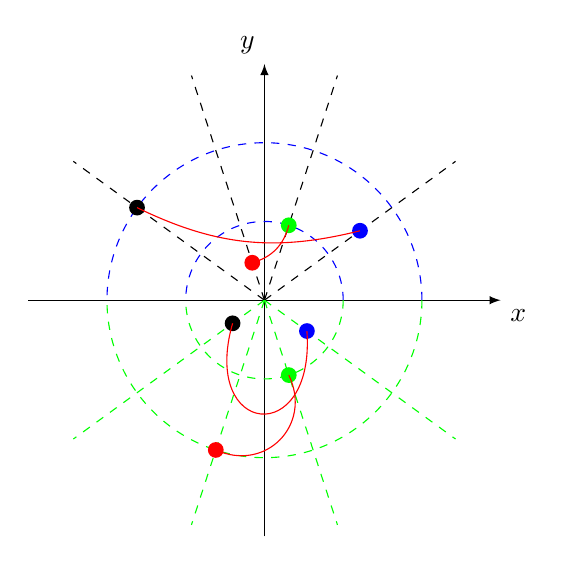
\begin{tikzpicture}
\draw[-latex] (-3,0) -- (3,0) node[pos=1,below right]{$x$};
\draw[-latex] (0,-3) -- (0,3) node[pos=1,above left]{$y$};

\draw[dashed] (0,0) -- (36:3);
\draw[dashed] (0,0) -- (72:3);
\draw[dashed] (0,0) -- (108:3);
\draw[dashed] (0,0) -- (144:3);

\draw[dashed, blue] (1,0) arc [start angle=0, end angle=180, radius = 1];
\draw[dashed, blue] (2,0) arc [start angle=0, end angle=180, radius = 2];

\coordinate (A) at (144:2);
\coordinate (B) at (108:1/2);
\coordinate (C) at (72:1);
\coordinate (D) at (36:1.5);

\fill[black] (A) circle [radius=0.1];
\fill[red] (B) circle [radius=0.1];
\fill[green] (C) circle [radius=0.1];
\fill[blue] (D) circle [radius=0.1];

\draw[red] (A) to [bend right=20pt] (D);
\draw[red] (B) to [bend right] (C);

\draw[dashed, green] (0,0) -- (-36:3);
\draw[dashed, green] (0,0) -- (-72:3);
\draw[dashed, green] (0,0) -- (-108:3);
\draw[dashed, green] (0,0) -- (-144:3);

\draw[dashed, green] (1,0) arc [start angle=0, end angle=-180, radius = 1];
\draw[dashed, green] (2,0) arc [start angle=0, end angle=-180, radius = 2];

\coordinate (IA) at (-144:0.5);
\coordinate (IB) at (-108:2);
\coordinate (IC) at (-72:1);
\coordinate (ID) at (-36:2/3);

\fill[black] (IA) circle [radius=0.1];
\fill[red] (IB) circle [radius=0.1];
\fill[green] (IC) circle [radius=0.1];
\fill[blue] (ID) circle [radius=0.1];

\draw[red] (IA) to [bend right=100, min distance=1.5cm] (ID);
\draw[red] (IB) to [bend right=70, min distance=0.7cm] (IC);
\end{tikzpicture}
\end{frame}


\begin{frame}
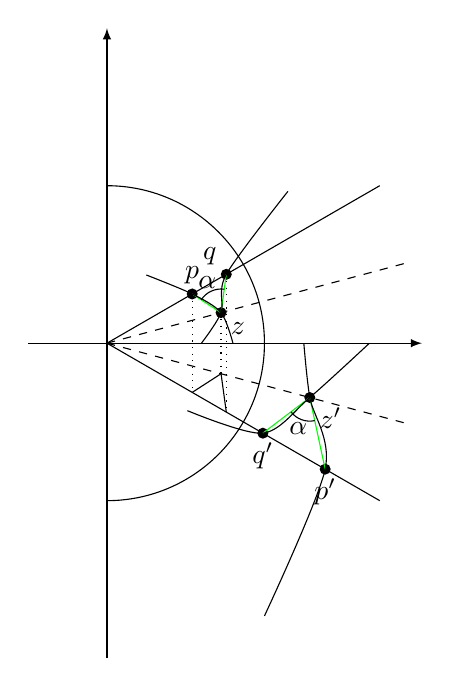
\begin{tikzpicture}[scale=2]
\draw[-latex] (-0.5,0) -- (2,0);
\draw[-latex] (0,-2) -- (0,2);

\draw[] (0,1) arc [start angle=90, end angle=-90, radius=1];

\draw[] (0,0) -- (30:2);
\draw[] (0,0) -- (-30:2);

\draw[dashed] (0,0) -- (15:2);
\draw[dashed] (0,0) -- (-15:2);

\fill[] (30:5/8) circle [radius=0.035] node[above]{$p$};
\fill[] (30:7/8) circle [radius=0.035] node[above left]{$q$};
\fill[] (15:6/8) circle [radius=0.035] node[below right]{$z$};

\draw[green] (15:6/8) -- (30:5/8);
\draw[green] (15:6/8) -- (30:7/8);

\draw plot [smooth] coordinates {(0:0.8)  (15:6/8)  (30:5/8) (60:0.5)}; 
\draw plot [smooth] coordinates {(0:0.6)  (15:6/8)  (30:7/8) (40:1.5)}; 

\fill[] (-30:1.6) circle [radius=0.035] node[below]{$p^\prime$};
\fill[] (-30:1.143) circle [radius=0.035] node[below]{$q^\prime$};
\fill[] (-15:4/3) circle [radius=0.035] node[below right]{$z^\prime$};

\draw[green] (-15:8/6) -- (-30:8/5);
\draw[green] (-15:8/6) -- (-30:8/7);

\draw[black] (-15:6/8) -- (-30:5/8);
\draw[black] (-15:6/8) -- (-30:7/8);

\draw[dotted] (30:5/8) -- (-30:5/8);
\draw[dotted] (30:7/8) -- (-30:7/8);
\draw[dotted] (15:6/8) -- (-15:6/8);

\draw plot [smooth] coordinates {(0:5/4)  (-15:8/6)  (-30:8/5) (-60:2)}; 
\draw plot [smooth] coordinates {(0:5/3)  (-15:8/6)  (-30:8/7) (-40:2/3)};

\coordinate (z) at (15:6/8);
\coordinate (p) at (30:5/8);
\coordinate (q) at (30:7/8);

\draw pic["$\alpha$",draw,-,angle eccentricity=1.4, angle radius=0.3cm]{angle=q--z--p};

\coordinate (iz) at (-15:8/6);
\coordinate (ip) at (-30:8/5);
\coordinate (iq) at (-30:8/7);

\draw pic["$\alpha$",draw,-,angle eccentricity=1.4, angle radius=0.3cm]{angle=iq--iz--ip};
\end{tikzpicture}
\end{frame}

\begin{frame}
\tdplotsetmaincoords{45}{30}
\begin{tikzpicture}[tdplot_main_coords, scale=1]
\draw[domain=-360:360,very thick,smooth,samples=500,variable=\t,red]
  plot ({sin(4*\t)*(1-(\t/360)^2)^(0.5)},\t/360,{cos(4*\t)*(1-(\t/360)^2)^0.5});
\draw[tdplot_screen_coords,very thin] (0,0) circle [radius=1];
\foreach \t in {0, 10, ..., 350}{
\begin{scope}
%\clip[] (-2,-2,0) rectangle (2,2,2);
\tdplotsetrotatedcoords{0}{\t}{0}
\draw[tdplot_rotated_coords,very thin] (0,0) circle [radius=1];
\tdplotsetrotatedcoords{90}{90}{0}
\draw[tdplot_rotated_coords,very thin] (0,0,{sin(\t)}) circle [radius={cos(\t)}];
\end{scope}}
\end{tikzpicture}
\end{frame}



\begin{frame}
\tdplotsetmaincoords{45}{45}
\begin{tikzpicture}[tdplot_main_coords]
\clip[tdplot_screen_coords] (-4.5,-3.5) rectangle (4.5,3.5);
\draw[-latex] (-10,0,0) -- (10,0,0) node[pos=1]{$x$};
\draw[-latex] (0,-10,0) -- (0,10,0) node[pos=1]{$y$};
%\draw[-latex] (0,0,-10) -- (0,0,10) node[pos=1]{$z$};

\newcommand{\PSz}[2]{(cos(####2)*cos(####1))}
\newcommand{\PSy}[2]{(cos(####2)*sin(####1))}
\newcommand{\PSx}[2]{(sin(####2))}

\newcommand{\ASx}[2]{(sin(####1))}
\newcommand{\ASy}[2]{(cos(####1)*sin(####2))}
\newcommand{\ASz}[2]{(cos(####1)*cos(####2))}

\newcommand{\Lx}[1]{(####1/360)}
\newcommand{\Ly}[1]{(sqrt(1-(####1/360)^2)*cos(3*####1))}
\newcommand{\Lz}[1]{(sqrt(1-(####1/360)^2)*sin(3*####1))}

\newcommand{\SPx}[2]{((####1)/(1-####2))}
\newcommand{\SPy}[2]{((####1)/(1-####2))}


\foreach \Vk in {0,10,...,350}{
%%% POLAR %%%
\draw[domain=0:360,smooth,samples=50,variable=\Vt,blue]  plot ({\PSx{\Vt}{\Vk}},{\PSy{\Vt}{\Vk}},{\PSz{\Vt}{\Vk}});
%%% AZIMUTH %%%
\draw[domain=0:360,smooth,samples=50,variable=\Vt,blue]  plot ({\ASx{\Vt}{\Vk}},{\ASy{\Vt}{\Vk}},{\ASz{\Vt}{\Vk}});
}

\foreach \Vk in {10,20,...,80}{
%%% AZIMUTHAL PROJECTION %%%
\draw[domain=0:360,smooth,samples=50,variable=\Vt,blue] 
plot ({\SPx{\ASx{\Vt}{\Vk}}{\ASz{\Vt}{\Vk}}},{\SPy{\ASy{\Vt}{\Vk}}{\ASz{\Vt}{\Vk}}});
%%% POLAR PROJECTION %%%
\draw[domain=0:360,smooth,samples=50,variable=\Vt,blue] 
plot ({-\SPx{\PSx{\Vt}{\Vk}}{\PSz{\Vt}{\Vk}}},{\SPy{\PSy{\Vt}{\Vk}}{\PSz{\Vt}{\Vk}}});
}
\foreach \Vk in {100,110,...,170}{
%%% AZIMUTHAL PROJECTION %%%
\draw[domain=0:360,smooth,samples=50,variable=\Vt,blue] 
plot ({\SPx{\ASx{\Vt}{\Vk}}{\ASz{\Vt}{\Vk}}},{\SPy{\ASy{\Vt}{\Vk}}{\ASz{\Vt}{\Vk}}});
%%% POLAR PROJECTION %%%
\draw[domain=0:360,smooth,samples=50,variable=\Vt,blue] 
plot ({\SPx{\PSx{\Vt}{\Vk}}{\PSz{\Vt}{\Vk}}},{\SPy{\PSy{\Vt}{\Vk}}{\PSz{\Vt}{\Vk}}});
}

\draw[domain=-360:360,smooth,samples=50,variable=\Vt,red]  plot ({\Lx{\Vt}},{\Ly{\Vt}},{\Lz{\Vt}});
\draw[domain=-360:360,smooth,samples=500,variable=\Vt,red] 
plot ({\SPx{\Lx{\Vt}}{\Lz{\Vt}}},{\SPy{\Ly{\Vt}}{\Lz{\Vt}}});

\end{tikzpicture}
\end{frame}

\begin{frame}
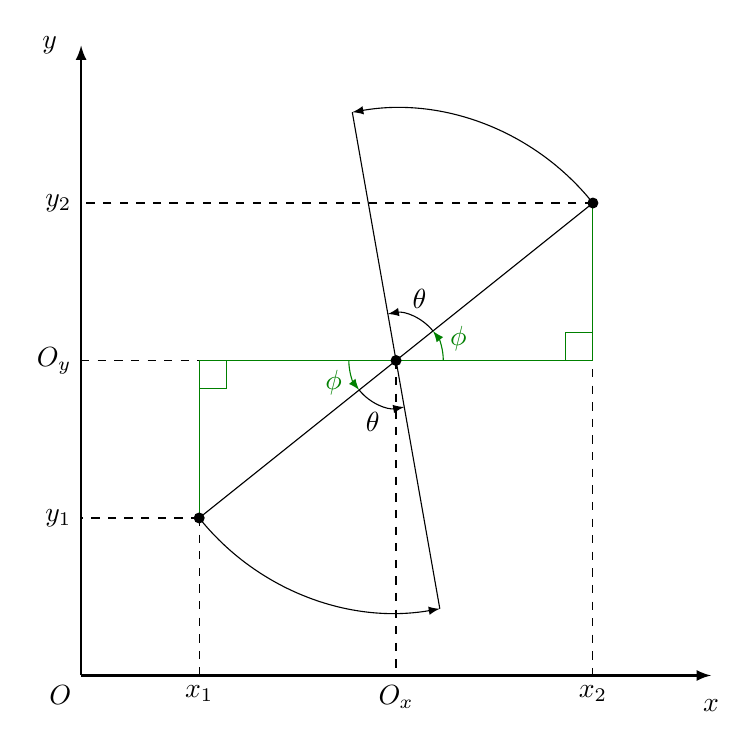
\begin{tikzpicture}
\draw[thick,-latex] (1,1) -- (1,9) node[pos=1,left=5pt] {$y$}; % y-axis
\draw[thick,-latex] (1,1) -- (9,1) node[pos=1,below=5pt] {$x$}; % x-axis
\node[below left] at (1,1) {$O$};
\coordinate (LI) at (2.5,3); % make coordinates for pic right angles
\coordinate (RI) at (7.5,7); % make coordinates for pic right angles
\coordinate (O) at (5,5); % make coordinates for pic right angles
\draw[] (LI) -- (RI); % initial radial line
\coordinate (LG) at (2.5,5); % make coordinates for pic right angles
\coordinate (RG) at (7.5,5); % make coordinates for pic right angles
\coordinate (LF) at (5.5559,1.8471); % coordinate
\coordinate (RF) at (4.4441,8.15292); % coordinate

\draw[] (LF) -- (RF); % final line

\draw[-latex] (LI) arc [start angle=180+38.6598, end angle=280, radius=3.20156]; % left arc
\draw[-latex] (RI) arc [start angle=38.6598, end angle=100, radius=3.20156]; % right arc

%%% ORIGIN DASHES %%%
\draw[dashed] (1,5) -- (5,5);
\node[left] at (1,5) {$O_y$};
\draw[dashed] (5,5) -- (5,1);
\node[below] at (5,1) {$O_x$};

%%% INITIAL DASHES %%%
\draw[dashed] (LI) -- (LI -| 1,0) node[pos=1,left] {$y_1$};
\draw[dashed] (LI) -- (LI |- 0,1) node[pos=1,below] {$x_1$};

%%% FINAL DASHES %%%
\draw[dashed] (RI) -- (RI -| 1,0) node[pos=1,left] {$y_2$};
\draw[dashed] (RI) -- (RI |- 0,1) node[pos=1,below] {$x_2$};


\draw[Green] (LI) -- (LG) -- (RG) -- (RI); % green stuff
\draw pic["$\phi$",-latex,draw,angle eccentricity=1.4, angle radius=0.6cm,Green]{angle=RG--O--RI}; % angle
\draw pic["$\phi$",-latex,draw,angle eccentricity=1.4, angle radius=0.6cm,Green]{angle=LG--O--LI}; % angle
\draw pic["",-,draw,angle eccentricity=1.4, angle radius=0.35cm,Green]{right angle=O--RG--RI}; % angle
\draw pic["",-,draw,angle eccentricity=1.4, angle radius=0.35cm,Green]{right angle=LI--LG--O}; % angle
\draw pic["$\theta$",-latex,draw,angle eccentricity=1.4, angle radius=0.6cm]{angle=RI--O--RF}; % angle
\draw pic["$\theta$",-latex,draw,angle eccentricity=1.4, angle radius=0.6cm]{angle=LI--O--LF}; % angle


%%% MUSTBE ON TOP %%%
\fill[] (O) circle [radius=0.07]; % origin of circle
\fill[] (LI) circle [radius=0.07]; % left point original
\fill[] (RI) circle [radius=0.07]; % right point original
\end{tikzpicture}
\end{frame}

\begin{frame}
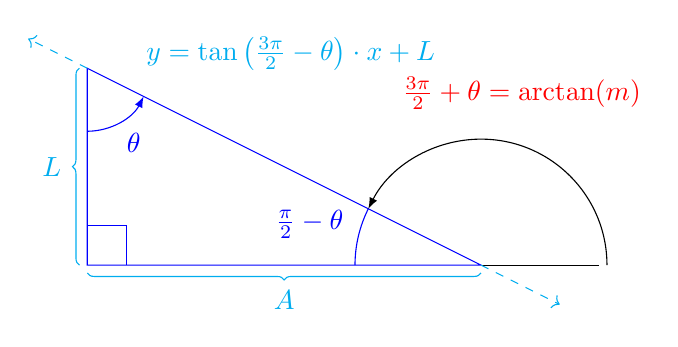
\begin{tikzpicture}[scale=0.5]
\coordinate (O) at (0,0); % origin
\coordinate (L) at (0,5); % height
\coordinate (A) at (10,0); % width
\draw[Blue] (O) -- (L) -- (A) -- cycle; % triangle base
\draw pic["",-,draw,angle eccentricity=1, angle radius=0.5cm,Blue]{right angle=A--O--L}; % right angle
\draw pic["$\theta$",-latex,draw,angle eccentricity=1.4, angle radius=0.8cm,Blue]{angle=O--L--A}; % angle theta
\draw pic["$\frac{\pi}{2}-\theta$",-,draw,angle eccentricity=1.4, angle radius=1.6cm,Blue]{angle=L--A--O}; % calculated angle [(pi/2) - theta]
\draw [decorate,decoration = {brace,mirror},cyan] (0,-0.2) --  (10,-0.2) node[pos=0.5,below=3pt,cyan]{$A$}; % auxillary aid to denote horizontal projection
\draw [decorate,decoration = {brace,},cyan] (-0.2,0) --  (-0.2,5) node[pos=0.5,left=3pt,cyan]{$L$}; % auxillary aid to denote vertical projection
\coordinate (C) at (10,0); % center of unit-circle angle
\coordinate (R) at (13,0); % right of unit-circle angle
\draw[black] (10,0) -- (13,0); % auxillary aid to denote unit-circle angle
\draw pic["\color{red}$\frac{3\pi}{2}+\theta=\arctan(m)\color{black}$",-latex,draw,angle eccentricity=1.4, angle radius=1.6cm]{angle=R--C--L}; % the unit circle angle
\draw[cyan,dashed,->] (0,5) -- (-1.5,5.75) node[pos=0.5,right=1cm]{$\color{cyan}y=\tan\left(\frac{3\pi}{2}-\theta\right)\cdot x+L$}; % left line extension
\draw[cyan,dashed,->] (10,0) -- (12,-1); % right line extension
\end{tikzpicture}
\end{frame}

\begin{frame}
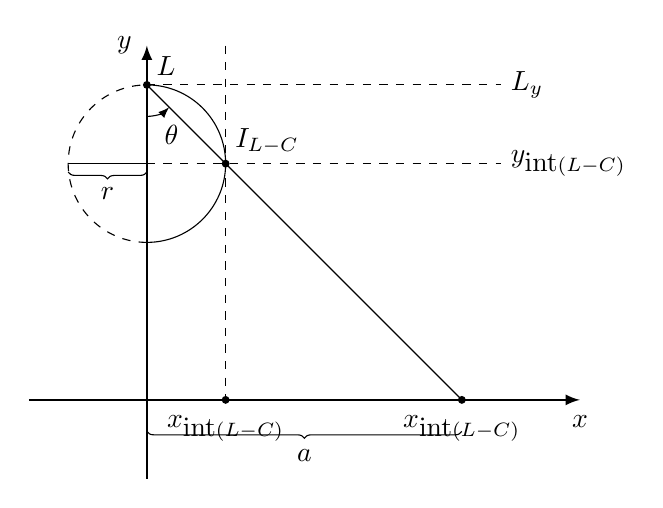
\begin{tikzpicture}[scale=0.5]
\draw[thick, -latex] (0,-2) -- (0,9); % y-axis
\draw[thick, -latex] (-3,0) -- (11,0); % x-axis
\draw[] (0,4) arc [start angle=-90, end angle=90, radius=2]; % circle right
\draw[dashed] (0,4) arc [start angle=-90, end angle=-270, radius=2]; % circle left
\draw[] (0,8) -- (8,0); % line right
\fill[] (0,8) circle [radius=0.1]; % L
\node[above right] at (0,8) {$L$};
\fill[] (2,6) circle [radius=0.1]; % C-intercept of L
\node[above right] at (2,6) {$I_{L-C}$}; % line-circle intercept
\fill[] (8,0) circle [radius=0.1]; % x-intercept of L
\draw[] (0,6) -- (-2,6); % radius
\draw[decoration={brace,raise=3pt},decorate] (0,6) -- (-2,6) node[pos=0.5, below=5pt]{$r$}; % radius label
\draw[dashed] (0,6) -- (9,6) node[pos=1,right]{$y_{\mbox{int}(L-C)}$}; % y intercept of (line-circle intercept)
\draw[dashed] (2,9) -- (2,0) node[pos=1,below=2pt]{$x_{\mbox{int}(L-C)}$}; % line-axis intercept vertical + label
\fill[] (2,0) circle [radius=0.1]; % line-axis intercept
\node[below=2pt] at (8,0) {$x_{\mbox{int}(L-C)}$}; % line-axis intercept label
\draw[dashed] (0,8) -- (9,8) node[pos=1,right]{$L_y$}; % y-intercept of point L
\node[below=2pt] at (11,0) {$x$}; % x-axis label
\node[left=2pt] at (0,9) {$y$}; % y-axis label
\draw[-latex] (0,7.2) arc [start angle=-90, end angle=-45, radius=0.8]; % angle arc
\node[below right=2pt] at (0.1,7.32) {$\theta$}; % angle denotation - theta
\draw [decorate,decoration = {brace,mirror}] (0,-0.8) --  (8,-0.8) node[pos=0.5,below=3pt]{$a$}; % auxillary aid to denote horizontal projection
\end{tikzpicture}
\end{frame}


\begin{frame}
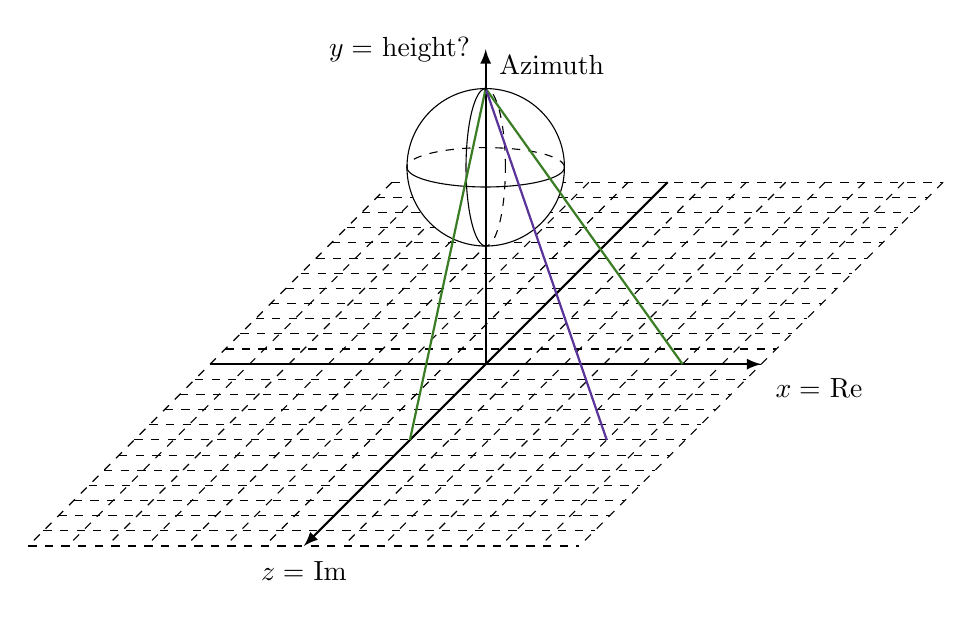
\begin{tikzpicture}[scale=0.5]

% A path that follows the edges of the current page
\tikzstyle{reverseclip}=[insert path={(current page.north east) --
  (current page.south east) --
  (current page.south west) --
  (current page.north west) --
  (current page.north east)}
]


%%% GRID LINES %%%
\foreach \x in {-7,-6,...,7}{
\draw[dashed] (\x, 0, -12) -- (\x, 0, 12);
}
\foreach \z in {-12,-11,...,12}{
\draw[dashed] (-7, 0, \z) -- (7, 0, \z);
}

\fill[white] (0,5) circle [radius=2];

%%% AXES %%%

%%% x-axis %%%
\draw[thick,-latex] (-7,0,0) -- (7,0,0) node[pos=1,below right=2pt]{$x=$ Re};

%%% y-axis %%%
\draw[thick,-latex] (0,0,0) -- (0,5+3,0) node[pos=1,left=2pt]{$y=$ height?};

%%% z-axis %%%
\draw[thick,-latex] (0,0,-12) -- (0,0,12) node[pos=1,below=2pt]{$z=$ Im};

%%% SPHERE CODE %%%
\draw[] (0,5) circle [radius=2];
\begin{scope} % fix so x>=0
\clip[] (0,-3+5) rectangle (3,3+5);
\draw[dashed] (0,0+5) circle [x radius=0.5, y radius=2];
\end{scope}
\begin{scope} % fix so x<0
\clip[] (0,-3+5) rectangle (-3,3+5);
\draw[] (0, 0+5) circle [x radius=0.5, y radius=2];
\end{scope}
\begin{scope} % fix so y<0
\clip[] (-3,0+5) rectangle (3,-3+5);
\draw[] (0,0+5) circle [x radius=2, y radius=0.5];
\end{scope}
\begin{scope} % fix so y>0
\clip[] (-3,0+5) rectangle (3,3+5);
\draw[dashed] (0,0+5) circle [x radius=2, y radius=0.5];
\end{scope}


%%% RAY TRACES %%%
\draw[OliveGreen,thick] (0,7,0) -- (5,0,0);
\draw[OliveGreen,thick] (0,7,0) -- (0,0,5);
\draw[RoyalPurple,thick] (0,7,0) -- (5,0,5);

%%% THINGS WHICH MUST BE ON TOP %%%
\fill[] (0,7,0) circle [radius=0.05]; % AZIMUTH POINT
\node[above right=2pt] at (0,7,0) {Azimuth};



\end{tikzpicture}
\end{frame}



\begin{frame}
\tdplotsetmaincoords{65}{165}
\begin{tikzpicture}[tdplot_main_coords,scale=2.5]

%%% axes %%%
% make dashed when inside or behind the riemann sphere
\draw[-latex] (-2,0,0) -- (2,0,0) node[pos=1,below left]{$x,\xi$}; % x-axis
\draw[-latex] (0,-3,0) -- (0,3,0) node[pos=1,below right]{$y,\eta$}; % y-axis
\draw[-latex] (0,0,-2) -- (0,0,2) node[pos=1,above right]{$z,\zeta$}; % z-axis

\draw[tdplot_screen_coords] (0,0) circle [radius=1]; % outer circle
%\tdplotsetrotatedcoords{0}{0}{0}
%\draw[tdplot_rotated_coords] (0,0) circle [radius=1]; % xy circle
\tdplotsetrotatedcoords{0}{90}{0}
\draw[tdplot_rotated_coords] (0,0) circle [radius=1]; % yz circle
%\tdplotsetrotatedcoords{90}{90}{0}
%\draw[tdplot_rotated_coords] (0,0) circle [radius=1]; % xz circle - not aesthetically pleasing.

\path[tdplot_rotated_coords,spath/save=name] (0,0) circle [radius=0.866];
\path[draw,spath/use={name, transform={shift={(2.5*0.5,4*0,4*0)}}}]; % circle by intersection of S by x=1/2
% draw circles first, so you can blank out the right parts
\path[tdplot_screen_coords,spath/save=name2] (0,0,0) circle [radius=0.025];
\path[fill,spath/use={name2, transform={shift={(2.5*0.5,2.5*0.5,2.5*0.71)}}}]; % point P
\draw[blue] (0,0,1) -- (1.71,1.71,0) node[below]{$z$}; % blue line

% base coords
\coordinate (O) at (0,0,0);
\node[above right] at (O) {$\scriptscriptstyle O$};
\coordinate (P) at (0.5,0.5,0.71);
\node[left] at (P) {$\scriptscriptstyle P$};
\coordinate (Q) at (0,0.5,0.71);
\node[above] at (Q) {$\scriptscriptstyle Q$};
\coordinate (Pp) at (0.5,-0.5,-0.71);
\node[below right] at (Pp) {$\scriptscriptstyle P^\prime$};
\coordinate (Qp) at (0,-0.5,-0.71);
\node[below] at (Qp) {$\scriptscriptstyle Q^\prime$};
\coordinate (N) at (0,0,1);
\node[above right,blue] at (N) {$\scriptscriptstyle N$};
\coordinate (S) at (0,0,0.71);
\node[left,blue] at (S) {$\scriptscriptstyle \zeta$};
\coordinate (n) at (0,0.5,0);
\node[below,blue] at (n) {$\scriptscriptstyle\eta$};
\coordinate (nS) at (0,0,-0.71);
\node[right,blue] at (nS) {$\scriptscriptstyle -\zeta$};
\coordinate (nn) at (0,-0.5,0);
\node[above,blue] at (nn) {$\scriptscriptstyle-\eta$};
\coordinate (B) at (0.5,0,0);
\node[above,red] at (B) {$\scriptscriptstyle B$};
% find w too...
\draw[dashed] (n) -- (Q) -- (S);
\draw[dashed] (nn) -- (Qp) -- (nS);
\draw[dashed] (Qp) -- (Q) -- (P) -- (Pp) -- (Qp);
\draw[blue,dashed] (N) -- (Pp);

\path[tdplot_screen_coords,spath/save=name2] (0,0,0) circle [radius=0.025];
\path[fill,spath/use={name2, transform={shift={(2.5*0,2.5*0,2.5*1)}}}]; % point N

\path[tdplot_screen_coords,spath/save=name2] (0,0,0) circle [radius=0.025];
\path[draw,spath/use={name2, transform={shift={(2.5*0.5,2.5*0,2.5*0)}}}]; % point B

\path[tdplot_screen_coords,spath/save=name2] (0,0,0) circle [radius=0.025];
\path[draw,spath/use={name2, transform={shift={(2.5*0.5,-2.5*0.5,-2.5*0.71)}}}]; % point Pp

\path[tdplot_screen_coords,spath/save=name2] (0,0,0) circle [radius=0.025];
\path[draw,spath/use={name2, transform={shift={(2.5*0,-2.5*0.5,-2.5*0.71)}}}]; % point Qp

\path[tdplot_screen_coords,spath/save=name2] (0,0,0) circle [radius=0.025];
\path[draw,spath/use={name2, transform={shift={(2.5*0,2.5*0.5,2.5*0.71)}}}]; % point Q

\path[tdplot_screen_coords,spath/save=name2] (0,0,0) circle [radius=0.025];
\path[draw,spath/use={name2, transform={shift={(2.5*0,2.5*0,-2.5*1)}}}]; % point SP
\node[blue,above right] at (0,0,-1) {$\scriptscriptstyle S$};

\end{tikzpicture}
\end{frame}


\begin{frame}
\centering
\tdplotsetmaincoords{40}{40}
\begin{tikzpicture}[tdplot_main_coords]

%%% DEFINITIONS %%%
\def \Vazi {0}

%%% OUTTER ELLIPSE %%%
\draw[very thin,tdplot_screen_coords] (0,0,0) circle(1);
\draw[-latex] (-3,0,0) -- (3,0,0) node[pos=1]{$x$};
\draw[-latex] (0,-3,0) -- (0,3,0) node[pos=1]{$y$};
\draw[-latex] (0,0,-3) -- (0,0,3) node[pos=1]{$z$};


%%% FOREACH LOOP %%%
\foreach \Vthe in {0, 10, ..., 350}{
%%% LONGITUTE %%%
\tdplotsetrotatedcoords{\Vazi-90}{\Vthe}{0}
\path[tdplot_rotated_coords,very thin,spath/save=pathname] (0,0,0) circle(1);
\path[draw,very thin,spath/use={pathname, transform={shift={({0},{0},{0})}}}];
%%% LATITUTE %%%
\tdplotsetrotatedcoords{\Vazi}{90}{0}
\path[tdplot_rotated_coords,very thin,spath/save=pathname] (0,0,0) circle [radius={cos(\Vthe)}];
\path[tdplot_rotated_coords,draw,very thin,spath/use={pathname, transform={shift={({0},{0},{sin(\Vthe)})}}}];
%%% MAGNETIC FIELD %%%
\foreach \Vdist in {20,40,60}{
\tdplotsetrotatedcoords{\Vazi-90}{\Vthe}{0}
\path[tdplot_rotated_coords,very thin,spath/save=pathname] ({1/cos(\Vdist)},0,0) circle({sqrt(1/(cos(\Vdist))^2-cos(\Vdist))});
\path[draw,very thin,spath/use={pathname, transform={shift={({0},{0},{0})}}}];
\tdplotsetrotatedcoords{\Vazi-90}{\Vthe}{90}
\path[tdplot_rotated_coords,very thin,spath/save=pathname] ({-sin(\Vdist)/cos(\Vdist)},0,0) circle({1/cos(\Vdist)});
\path[draw,very thin,spath/use={pathname, transform={shift={({0},{0},{0})}}}];
\path[tdplot_rotated_coords,very thin,spath/save=pathname] ({sin(\Vdist)/cos(\Vdist)},0,0) circle({1/cos(\Vdist)});
\path[draw,very thin,spath/use={pathname, transform={shift={({0},{0},{0})}}}];
}

}
\end{tikzpicture}
\end{frame}



\end{document}
